\title{Graphs  - Recitation 9} 
\documentclass{article}


\usepackage[utf8]{inputenc}
\usepackage[a4paper, total={6in, 9in}]{geometry}
\usepackage{braket}
\usepackage{xcolor}
\usepackage{amsmath}
\usepackage{amsfonts}
\usepackage{tikz}
\usepackage{svg}
\usepackage{graphicx}
\usepackage{media9}
\usepackage{float}
\usetikzlibrary{calc}
\usepackage{array}
\usepackage[ruled,vlined,linesnumbered]{algorithm2e}

\usepackage[
backend=biber,
style=alphabetic,
sorting=ynt
]{biblatex}



\newcommand{\commentt}[1]{\textcolor{blue}{ \textbf{[COMMENT]} #1}}
\newcommand{\ctt}[1]{\commentt{#1}}
\newcommand{\prb}[1]{ \mathbf{Pr} \left[ {#1} \right]}
\newcommand{\onotation}[1]{\(\mathcal{O} \left( {#1}  \right) \)}
\newcommand{\ona}[1]{\onotation{#1}}
\newcommand{\nvar}[2]{ \( #1_{1}, #1_{2} ... #1_{#2}  \) }
%\newenvironment{proof}[0]{\paragraph{Proof.}}{}
%\newenvironment{remark}[0]{\textit{remark}}{}
\newenvironment{cor}[0]{\paragraph{Corollary.}}{}
\newenvironment{example}[0]{\paragraph{Example.}}{}
%\newenvironment{thm}[0]{\paragraph{Theorem.}}{}
\newtheorem{prop}{Proposition}
\newtheorem{ex}{Exercise}
\newtheorem{sol}{Solution}
\newtheorem{theorem}{Theorem} 		
\newtheorem{thm}{Theorem}[section]
\newtheorem{conj}[thm]{Conjecture} 	
\newtheorem{lemma}[thm]{Lemma}
\newtheorem{corollary}[thm]{Corollary} 
\newtheorem{claim}[thm]{Claim}
\newtheorem{proposition}[thm]{Proposition}
\newtheorem{definition}{Definition} 
\newtheorem{remark}{Remark}
 


% \addbibresource{sample.bib} %Import the bibliography file
\begin{document}    
\maketitle
\usetikzlibrary{positioning, arrows}
\tikzset{main node/.style={circle,draw,minimum size=0.8cm,inner sep=0pt},}
\tikzset{edge/.style = {->,> = latex'}}

\iffalse
\newtheorem{prop}{Proposition}
\newtheorem{ex}{Exercise}
\newtheorem{sol}{Solution}
\newtheorem{theorem}{Theorem} \newtheorem{thm}{Theorem}[section]
\newtheorem{conj}[thm]{Conjecture} \newtheorem{lemma}[thm]{Lemma}
\newtheorem{corollary}[thm]{Corollary} \newtheorem{claim}[thm]{Claim}
\newtheorem{proposition}[thm]{Proposition}
\newtheorem{definition}{Definition} \newtheorem{remark}{Remark}
   
\pagestyle{empty}

\setlength{\textwidth}{6.5in}
\setlength{\evensidemargin}{0.0in}
\setlength{\oddsidemargin}{0.0in}
\setlength{\topmargin}{-0.25in}
\setlength{\textheight}{9.0in}
\setlength{\baselineskip}{1.3\baselineskip}
\setlength{\parindent}{.0in}
\fi
\tikzset{
node of list/.style = { 
             draw, 
             fill=orange!20, 
             minimum height=6mm, 
             minimum width=6mm,
             node distance=6mm
   },
link/.style = {
     -stealth,
     shorten >=1pt
     },
array element/.style = {
    draw, fill=white,
    minimum width = 6mm,
    minimum height = 10mm
  }
}

\def\LinkedList#1{%
  \foreach \element in \list {
     \node[node of list, right = of aux, name=ele] {\element};
     \draw[link] (aux) -- (ele);
     \coordinate (aux) at (ele.east);
  } 
}



%%%%%%%%%%%%%%%%%%%%%%%%%%%%%%%%%%%%%%%%%%%%%%%%%%%%%%%%%%%%



%%%%%%%%%%%%%%%%%%%%%%%%%%%%%%%%%%%%%%%%%%%%%%%%%%%%%%%%%%%%

%\vspace{0.2in}

\section{Graphs}
This is an important section, as you'll be seeing graph's A LOT, both in this course and in courses to follow. 

\subsection{Definitions, Examples and Basics}

\begin{figure}[h]
\begin{subfigure}[b]{0.65\textwidth}
\begin{definition}
A \textbf{non-directed graph} $G$ is a pair of two sets - $G=(V, E)$ - $V$ being a set of vertices and $E$ being a set of couples of vertices, which represent edges ("links") between vertices.
\end{definition}

\textbf{Example}: $G= (\{1,2,3,4\},\ \{\{1,2\}, \{1,3\}, \{3,4\}\})$ is the following graph:\\ 
\end{subfigure}
\begin{subfigure}[b]{0.05\textwidth}
  \
\end{subfigure}
  \begin{subfigure}[b]{0.25\textwidth}
    \begin{tikzpicture}
\node[main node](1){$1$};
\node[main node](2)[below = 1cm of 1]{$2$};
\node[main node](3)[right = 1cm of 1]{$3$};
\node[main node](4)[below = 1cm of 3]{$4$};

\path[draw, thick]
(1) edge node {} (2)
(1) edge node {} (3)
(3) edge node {} (4);
\end{tikzpicture}
\end{subfigure}
\end{figure}
\begin{figure}[h]
\begin{subfigure}[b]{0.65\textwidth}
\begin{definition}
A \textbf{directed graph} $G$ is a pair of two sets - $G=(V, E)$ - $V$ being a set of vertices and $E\subseteq V\times V$ being a set of directed edges ("arrows") between vertices.
\end{definition}
\textbf{Example}: $G=(\{1,2,3,4\},\ \{(1, 2), (1, 4), (4, 1), (4,3)\})$ is the following graph (note that it has arrows): \\ 
\end{subfigure}
\begin{subfigure}[b]{0.05\textwidth}
  \
\end{subfigure}
  \begin{subfigure}[b]{0.25\textwidth}
    \begin{tikzpicture}
\node[main node](1){$1$};
\node[main node](2)[below = 1cm of 1]{$2$};
\node[main node](3)[right = 1cm of 1]{$3$};
\node[main node](4)[below = 1cm of 3]{$4$};

\draw[edge] (1) to (2);
\draw[edge] (1) to (4);
\draw[edge] (4) to (1);
\draw[edge] (4) to (3);
\end{tikzpicture}
\end{subfigure}
\end{figure}
Now that we see graphs with our eyes, we can imagine all sorts of uses for them... For example, the can represent the structure of the connections between friends on facebook, or they can even represent which rooms in your house have doors between them.

\begin{remark}
Note that directed graphs are a \textbf{generalization} of non-directed graphs, in the sense that every non-directed graph can b represented as a directed graph. Simply take every non-directed edge $\{v,u\}$ and turn it into two directed edges $(v,u), (u,v)$. 
\end{remark}

\begin{remark}
Note that most of the data structures we discussed so far - Stack, Queue, Heap, BST - can all be implemented using graphs.
\end{remark}

Now let's define some things in graphs:

\begin{definition} (Path, circle, degree)
\begin{enumerate} 
\item A \textbf{simple path} in the graph $G$ is a series of unique vertices (that is, no vertex appears twice in the series) $v_1, v_2, ..., v_n$ that are connected with edges in that order. 
\item A \textbf{simple circle} in the graph $G$ is a simple path such that $v_1 = v_n$. 
\item The \textbf{distance} between two vertices $v,u\in V$ is the length of the shortest path between them ($\infty$ if there is no such path).
\end{enumerate}
\end{definition}

\begin{remark}
Note that for all $u,v,w\in V$ the triangle inequality holds regarding path lengths. That is:
$$dist(u,w)\leq dist(u,v) + dist(v, w)$$
\end{remark}

\begin{definition} (connectivity)
\begin{enumerate}
\item A \textbf{connected component} is a subset $U \subseteq V$ of maximal size in which there exists a path between every two vertices. 
\item A graph $G$ is said to be a \textbf{connected} graph if it only has one connected component.
\end{enumerate}
\end{definition}
\begin{figure}[h]
  \begin{subfigure}[b]{0.4\textwidth} 
An \textbf{example} of a non-connected graph: \\ \\ \\  \\
\end{subfigure}
\begin{subfigure}[b]{0.05\textwidth}
  \
\end{subfigure}
\begin{subfigure}[b]{0.25\textwidth}
\begin{tikzpicture}
\node[main node](1){$1$};
\node[main node](2)[below = 1cm of 1]{$2$};
\node[main node](3)[right = 1cm of 1]{$3$};
\node[main node](4)[below = 1cm of 3]{$4$};

\draw[edge] (1) to (2);
\draw[edge] (3) to (4);
\end{tikzpicture}
\end{subfigure}
\end{figure}

\begin{prop}
Let $G=(V,E)$ be some graph. If $G$ is connected, then $|E| \geq |V|-1$
\end{prop}

\begin{proof}
We will perform the following cool process: Let $\{e_1,...,e_m\}$ be an enumeration of $E$, and let $G_0=(V,\emptyset)$. We will build the graphs $G_1, G_2,... G_m=G$ by adding edges one-by-one. Formally, we define - 
$$\forall i\in[m]\ \ G_i=(V,\{e_1,...,e_i\})$$
$G_0$ has exactly $|V|$ connected components, as it has no edges at all. Then $G_1$ has $|V|-1$. From there on, any edges does one of the following:
\begin{enumerate}
    \item Keeps the number of connected components the same (the edge closes a cycle)
    '\item Lowers the number of connected components by $1$ (the edges does not close a cycle)
\end{enumerate}

So in general, the number of connected components of $G_i$ is $\geq |V|-i$. 
Now, if $G_m=G$ is connected, it has just one connected component! This means:
$$1 \geq |V| - |E|\ \implies \ |E|\geq|V|-1$$

\end{proof}


\subsection{Graph Representation}

Okay, so now we know what graphs are. But how can we represent them in a computer? There are two mainly options. The first one is by \textbf{array of adjacency lists}. Given some graph $G$, every slot in the array will contain a linked list. Each linked list will represent a list of some node's neighbors. The second option is to store edges in an \textbf{adjacency matrix}, a $ |V| \times |V| $ binary matrix in which the $v,u$-cell eqauls $1$ if there is an edge connecting $u$ to $v$. In the example below the matrix is denoted by $A_{G}$. Note that the running time anlysis might depands on the underline representaion.     

\textbf{Question.} What is the memmory cost of each of the representations? Note that while holding an adjacency matrix requires to store $|V|^2$ bits regardless the size of $E$, Mainting the edges by adjacency lists costs linear memmory at number of edges and therefore only $ \Theta \left(  |V| + |E| \right) $ bits. 

\paragraph{Example.} Consider the following directed graph:
\begin{figure}[h]
  \centering
  \begin{subfigure}[b]{0.25\textwidth}
    \begin{tikzpicture}
      \node[main node](1){$1$};
      \node[main node](2)[below = 1cm of 1]{$2$};
      \node[main node](3)[right = 1cm of 1]{$3$};
      \node[main node](4)[below = 1cm of 3]{$4$};

      \draw[edge] (1) to (2);
      \draw[edge] (1) to (4);
      \draw[edge] (4) to (1);
      \draw[edge] (4) to (3);
      \draw[edge] (1) to (3);
      \draw[edge] (3) to (1);
    \end{tikzpicture}  
    \\ \\  
  \end{subfigure} 
  \begin{subfigure}[b]{0.49\textwidth}
    \begin{tikzpicture}
      \foreach \index/\list in {1/{2,3,4,null}, 2/{null}, 3/{1, null}, 4/{1, 3, null}} {
	\node[array element] (aux) at (0,-\index) {\index};
	\LinkedList{\list}
      }
    \end{tikzpicture}  
  \end{subfigure}
  \caption{ Persenting $G$ by array of adjacency lists.  }
\end{figure}

%Its representation will be: \\ \\

\begin{figure}[h]
  \centering
  \begin{subfigure}[b]{0.25\textwidth}
        \begin{tikzpicture}
\node[main node](1){$1$};
\node[main node](2)[below = 1cm of 1]{$2$};
\node[main node](3)[right = 1cm of 1]{$3$};
\node[main node](4)[below = 1cm of 3]{$4$};

\draw[edge] (1) to (2);
\draw[edge] (1) to (4);
\draw[edge] (4) to (1);
\draw[edge] (4) to (3);
\draw[edge] (1) to (3);
\draw[edge] (3) to (1);
\end{tikzpicture} \\ 
  \end{subfigure}
\begin{subfigure}[b]{0.49\textwidth}       
  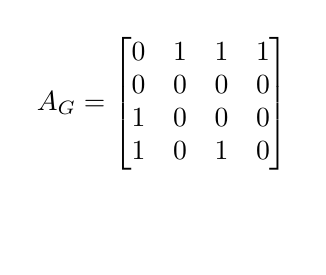
\begin{tikzpicture}
    \node (1) at (0,0) { };
    \node  (2) at (1,1.7) { $ A_{G} = 
	  \begin{bmatrix}
	0 & 1 & 1 & 1\\
	0 & 0 & 0 & 0\\
	1 & 0 & 0 & 0\\
	1 & 0 & 1 & 0
	\end{bmatrix}
      $ };
      \end{tikzpicture}
\end{subfigure}
\caption{ Presenting $G$ by adjacency matrix. }
\end{figure}

\subsection{Breadth First Search (BFS)}

One natural thing we might want to do is to travel around inside a graph. That is, we would like to visit all of the vertices in a graph in some order that relates to the edges. \\ 
One reason to want such a thing is the following objective: Given some start vertex $v$, we would like to know how long is the shortest path from $s$ to every vertex $v\in V$. \\ 
For this we present the following algorithm, which receives the connected graph $G$ and the starting node $s$ as input. Note that in addition to our definition of the graph $G$, we will now also save some property $dist$ for every vertex, and also a flag called $visited$.  (Now read the algorithm, it may be in the next page because LaTeX is dumb...)

\begin{algbox}{BFS($G, s$)}
  \begin{algorithm}[H]
    \For {$v\in V$}{
 	set $v.dist \leftarrow \infty$, $v.visited \leftarrow False$
      }
 set $s.dist\leftarrow 0$ \\
 $Q\leftarrow$ new Queue \\ 
 $Q$.Enqueue($s$) \\
 $s$.visited $\leftarrow$ True
 \While {$Q$ is not empty} {
 $u\leftarrow Q$.Dequeue() \\
	\For {neighbor $w$ of $u$}{
	\If {$w$.visited is False}{
		 $w$.visited$\leftarrow$ True \\
		 $w$.dist $\leftarrow \min(w$.dist, $u$.dist$+1)$ \\
		 $Q$.Enqueue($w$)

	      }
	}
      }
  \end{algorithm}
\end{algbox}
\textbf{Example}: In the tirgul video...

\underline{Correctness}: The example should be enough to explain the correctness. A concrete proof can be found in the book, page 597.


\underline{Runtime}: We can analyse the runtime line-by-line:
\begin{itemize}
\item Lines 1-2: $|V|$ operations, all in $O(1)$ runtime, for a total of $O(|V|)$.
\item Lines 3-6: $O(1)$
\item Lines 7-8: First we need to understand the number of times the $while$ loop iterates. We can see that every vertex can only enter the queue ONCE (since it is then tagged as "visited"), and therefore it runs $\leq |V|$ times. All operations are $O(1)$, and we get a total of $O(|V|)$. 
\item Lines 9-13: Next, we want to understand the number of times this $for$ loop iterates. 
The for loop starts iterating once per vertex, and then the number of its iterations is the same as the number of neighbours that this vertex has. Thus, it runs $O(|E|)$ times.
\end{itemize}
So all in all we get a runtime of $O(|V|+|E|)$

\subsection{Usage of BFS}
Now we have in our hands a way to travel  through a graph using the edges. How else can we use it?\\ \\ 
\textbf{Exercise}: Present and analyse an algorithm $CC(G)$ which receives some undirected graph $G$ and outputs the number of connected components in $G$ in $O(|V|+|E|)$. \\

\textbf{Solution}: Consider the following algorithm: (Now read the algorithm, it may be in the next page because LaTeX is dumb...)
\begin{algbox}{CC($G$)}
  \begin{algorithm}[H]
     count $\leftarrow 0$
     \For {$v\in V$ }{
	\If {$v$.visited = False} {
	  count$\leftarrow$count$+1$ \\
	  BFS($G, v$)
	}
      }
	\Return count
  \end{algorithm}
\end{algbox}
\underline{Correctness}: We know that given some vertex $v\in V$, $BFS(G, v)$ marks all of the nodes in the connected component of $v$ as marked (Since $BFS$ marks all vertices in a connected graph). So each time that $BFS$ is invoked, it is because some vertex $v$ has not been visited, meaning it is not in the same connected component as any of the previous vertices. \\

\underline{Runtime}: Let's denote all of the connected components in $G$ by $(G_i=(V_i , E_i))_{i=1}^k$. For each connected component, the runtime of $BFS$ will be $O(|V_i|+|E_i|)$. So all in all, we get $O(|V|+|E|)$.

\subsection{Correctness}

We must not forget to prove BFS's correctness! Specifically, we want to prove that after calling $BFS(G, s)$, we have that for all nodes $v$ in $s$'s connected component, $v$.visited = True. We will prove something stronger:

\begin{prop}
Let $G=(V,E)$ and let $s\in V$. For each $v\in V$ denote $d_v=dist(s, v)$. 
After $BFS(G,s)$ is called, all nodes with $d_v=k$ are inserted to the queue, and they are insterted before all nodes with $d_v=k+1$.
\end{prop}

\begin{proof}
We prove this by induction on $k$. 

\underline{Base}: $k=0$. Only $d_s=0$, and it is in fact inserted first.

\underline{Hypothesis}: Assume correctness for all $l<k$.

\underline{Step}: Let $v$ be a node such that $d_v=k$ (if there is no such $v$ we are done). By I.H for $k-1$, we know that all nodes $u$ with $d_u=k-1$ were inserted into the queue by now. By definition of the distance function, there exists some node $u_0$ such that $d_{u_0}=k-1$ and $(u_0,v)\in E$. When $u_0$ is dequeued, $v$ is inserted into the queue. 

So far we have proved that all nodes of distance $k$ are eventually inserted to the queue. We still need to show that this is done before all nodes of distance $k+1$. 

Assume towards contradiction that $v$ is inserted before $w$, where $d_v=k+1,\ d_w=k$. If $v$ was accessed through $u$ and $w$ was accessed through $x$, then $d_u = k$ and $d_x=k-1$. Since a queue is LIFO, we get that $u$ was inserted before $x$, but this is a contradiction to the I.H.


\end{proof}

\begin{remark}
If $v$ is not in the connected component of $s$ then $d_v=\infty$.
\end{remark}


\begin{corollary}
After $BFS(G,s)$ is run, $v$.visited = True for all $v$ in the connected component of $s$!
\end{corollary}

\subsection{Depth First Search (DFS)}
\begin{algbox}{DFS($G$)}
  \begin{algorithm}[H]
   \bf{DFS}( $G$): \\
    \For {$v\in V$}{
 	$vi$.visited $\leftarrow False$
    }
    time $ \leftarrow 1 $
    \For {$v\in V$}{
      \If { not $v$.visited } {
	$\pi \left( v \right) v \leftarrow $ null \\ 
	Explore( $G,v$ ) 
     } 
   }

  \end{algorithm}

  \begin{algorithm}[H]
    \bf{Explore}($G,v$): \\
    \For {$\left( v,u \right) \in E  $}{
      Previsit($v$)
      \If { not $u$.visited } {
	$ \pi \left( u \right) \leftarrow v $ \\ 
	Explore( $G, u$ ) 
      }
      Postvisit($v$)
    }
  \end{algorithm}
  \begin{algorithm}[H]
    \bf{Previsit}($v$): \\
    pre($v$) $\leftarrow $ time \\
    time $\leftarrow$ time $+1$
  \end{algorithm}
 \begin{algorithm}[H]
   \bf{Postvisit} ($v$): \\ 
    post($v$) $\leftarrow $ time \\
    time $\leftarrow$ time $+1$
  \end{algorithm}


\end{algbox}

% \printbibliography 
\end{document}
